\subsection{Data cleaning}
\fancyhead{}    % reset header
\fancyhead[R]{Data cleaning}
Nella prima fase di ingegnerizzazione dei dati ci siamo soffermati sul data cleaning, ovvero siamo andati ad analizzare i dati valutando se ci fossero valori nulli o non validi.
Da un analisi preliminare dei dati a nostra disposizione è risultato che:

\begin{figure}[h]
    \centering
    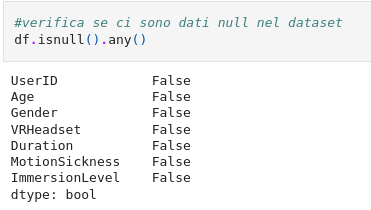
\includegraphics[width=0.75\textwidth]{MetaClassAI_Documentazione/3/img/ValoriNULLDataset.png}
    \caption{Esempio di verifica dei dati per valori nulli}
    \label{fig:verifica-null-dataset}
\end{figure}

\begin{figure}[h]
    \centering
    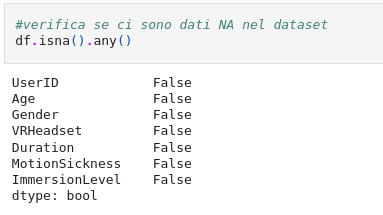
\includegraphics[width=0.75\textwidth]{MetaClassAI_Documentazione/3/img/ValoriNADataset.png}
    \caption{Esempio di verifica dei dati per valori N/A}
    \label{fig:verifica-NA-dataset}
\end{figure}
Come si può notare, non sono presenti dati nulli o invalidi tra quelli presenti, per cui non sono state necessarie tecniche di Data cleaning.
